\section{Реализация}

\subsubsection*{Необходимо реализовать:}
\begin{itemize}
    \item Структуру автоматона, функции для работы с ним
    \item Общие операции для решеток (join, meet, strictEquals, ...)
    \item Операции на строках (length, concat, substring, ...)
    \item Оператор замыкания (widening)
\end{itemize}

\subsubsection*{Дополнительные требования:}
\begin{itemize}
    \item Есть тестовый датасет из 23 и 62 реальных проектов
    \item Время исполнения не должно увеличиться более чем на $20\%$
    \item Потребление памяти не должно увеличиться более чем на $10\%$
\end{itemize}

\newpage
\subsection{Структура}
Сама структура автомата базовая - есть вершины (states) и переходы между ними. Некоторые из стейтов помечены как начальные или как конечные. На переходах стоят строки или символ $\top$, обозначающий любую строку

\subsubsection*{union}
Основной операцией является объединение автоматов. С её помощью находим наименьший язык, содержащий оба, порождаемых автоматами

Реализаиця простая: создаем общее начальное состояние, проводим из него переходы с пустой строкой в начальные состояния двух объединяемых автоматов. Затем минимизируем полученный автомат (чуть ниже описана функция minimize)

\subsubsection*{intersect}
Еще одной важной операцией является пересечение автоматов. Она позволяет понять, есть ли в двух алфавитах общие слова. А также находить наибольший общий подъязык

Реализуется она при помощи операций дополнения и объединения, то есть по формуле \[A \cap B = S / ((S / A) \cup (S / B))\]

Дополнение строится таким образом - выписываем все возможные переходы в обоих автоматах, а затем для каждого переходы между двумя вершинами заменяются на дополнение к этим переходам

\subsubsection*{subset}
Проверка на то, что один язык полностью содержит другой. Реализуется с помощью дополнения и пересечения по формуле
\[A \subset B <=> (S / B) \cap A = \emptyset\]

\subsubsection*{minimize}
Убирает лишние вершины и переходы. Например может произойти так, что из одной вершины ведут 2 перехода с одинаковой строкой. Тогда можно упростить автомат так, чтобы склеились 2 вершины в одну. Также избавляемся от переходов по пустой строке

Алгоритм минимизации такой - сначала проверяем, является ли автомат детерменированным, то есть что нет двух исходящих переходов из одной вершины с одинаковыми символами на них. А также что нет пустых переходов. Если есть, то склеиваем эти 2 вершины. Это операция детерменирования

Затем, чтобы избавиться от двух одинаковых входящих переходов, мы делаем reverse, то есть перенаправляем все ребра и помечаем конечные вершины начальными и наоборот. Теперь вызываем еще раз determinize. Повторив еще раз reverse + determinize, получим начальный автомат, но без лишних переходов и вершин

Последним шагом удаляем те вершины, из которых нельзя попасть в финальные. Таким образом получим упрощенную версию того же самого автомата

\newpage
\subsection{Операции для решеток}
Операции join и meet аналогичны union и intersect для автоматов. Остается только разобрать случаи, когда один из аргументов $\top$ или $\bot$. 

\subsubsection*{strictEquals}
Проверяем, что 2 автомата порождают одинаковые языки. В общем случае можем проверить то, что один язык включается в другой (subset) и наоборот. Однако операция пересечения слишком громоздкая (нужно сделать 3 раза дополнение), поэтому для конечных языков проще выписать 2 порождаемых языка и проверить их на соответствие. Язык является конечным, если в нем нет $\top$ переходов и циклов

\subsubsection*{equals}
В отличие от strictEquals, equals проверяет то, что есть хоть одно общее слово. Опять это можно сделать при помощи пересечения, то есть что пересечение не пусто. Но для конечных лучше сравнивать языки





\newpage
\subsection{Операции на строках}
\subsubsection*{Length}
Возвращает интервал $[c_1, c_2]$, такой что $c_1 \leq |s| \leq c_2$. При этом если $s$ содержит в себе цикл, или же содержит в себе переход, на котором стоит $\top$, то есть любая строка, то максимальная длина будет сколь угодно большой. Минимальная при этом заменяет все топы на пустые строки
\begin{figure}[H]
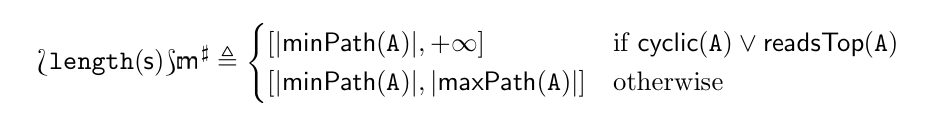
\includegraphics[width=\textwidth]{images/tarsis-length.png}\hfill
\end{figure}

Для подсчета длины запускаем DFS из начальных стейтов. При вхождении в конечную, считаем длину пути (заменяя $\top$ на $0$ или $+\infty$ соответственно) и пересчитываем максимальную и минимальную длину

Если автомат содержит в себе цикл, то с помощью DFS мы его найдем и максимальная длина пути будет бесконечной, так как можно по этому циклу крутиться сколь угодно много раз

\subsubsection*{Concat}
При конкатенации достаточно добавить для первого автомата одну дополнительную конечную вершину, в которую будут вести переходы с пустой строкой из конечных вершин первого, а затем из нее ведут переходы в начальные вершины второго автомата. Далее стоит минимизировать полученный автомат, чтобы избавиться от пустых ребер

\newpage
\subsubsection*{Contains}
Абстрактная семантика contains должна возвращать значение true, если любая строка из A' содержится в любой строке из A, значение false, если какая-то строка из A' не содержится в какой-то строке из A и \{true, false\} ($\top$) в остальных случаях
\begin{figure}[H]
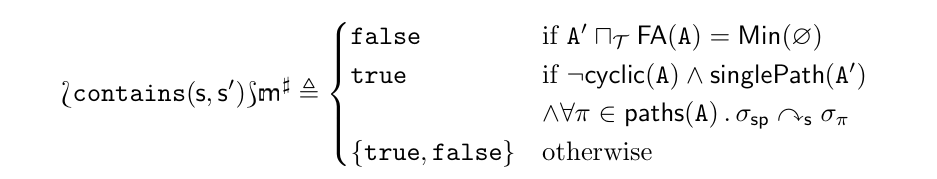
\includegraphics[width=\textwidth]{images/tarsis-contains.png}\hfill
\end{figure}
Для начала определим, в каком случае нужно возвращать false. Для этого определим фактор-автоматон FA(A), который принимает все подстроки A. Для этого нужно просто пометить все стейты конечными. Затем пересечь FA(A) и A', чтобы проверить, что никакая подстрока любой строки из A не является строкой из A'

Теперь, в каком случае true. Если A' содержит 2 слова, ни одно из которых не является префиксом другого, то они оба не могут быть одновременно префиксами какого-либо слова из A. Значит все слова в A' должны быть по цепочке включены друг в друга. Или же автомат для них выглядит как путь, некоторые вершины на котором конечные. И в этом случае достаточно проверить, что самое длинное слово входит во все слова из A, тогда и его префиксы будут

Во всех остальных случаях точного ответа нет, поэтому возвращаем $\top$

\newpage
\subsubsection*{IndexOf}

\begin{figure}[H]
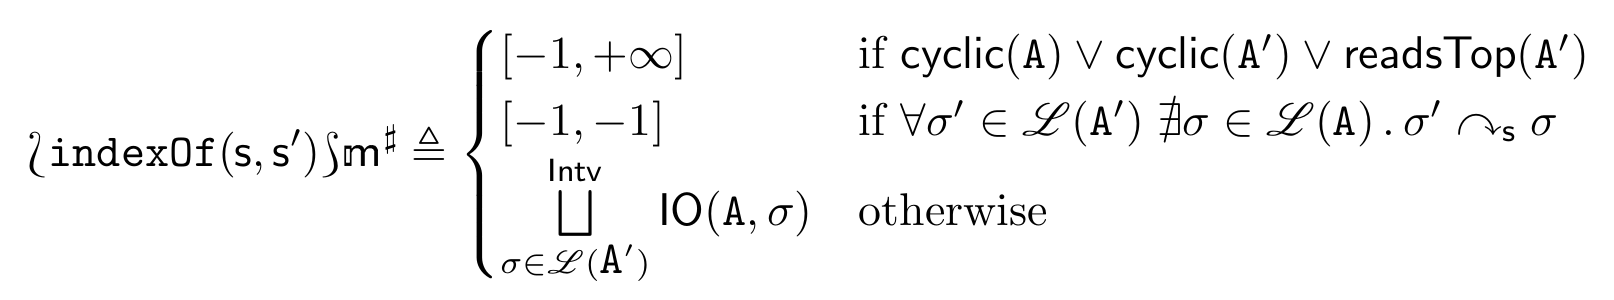
\includegraphics[width=\textwidth]{images/tarsis-indexOf.png}\hfill
\end{figure}

\newpage
\subsubsection*{Substr}
\begin{figure}[H]

\includegraphics[width=\textwidth]{images/tarsis-substr.png}\hfill
\end{figure}

\begin{figure}[H]
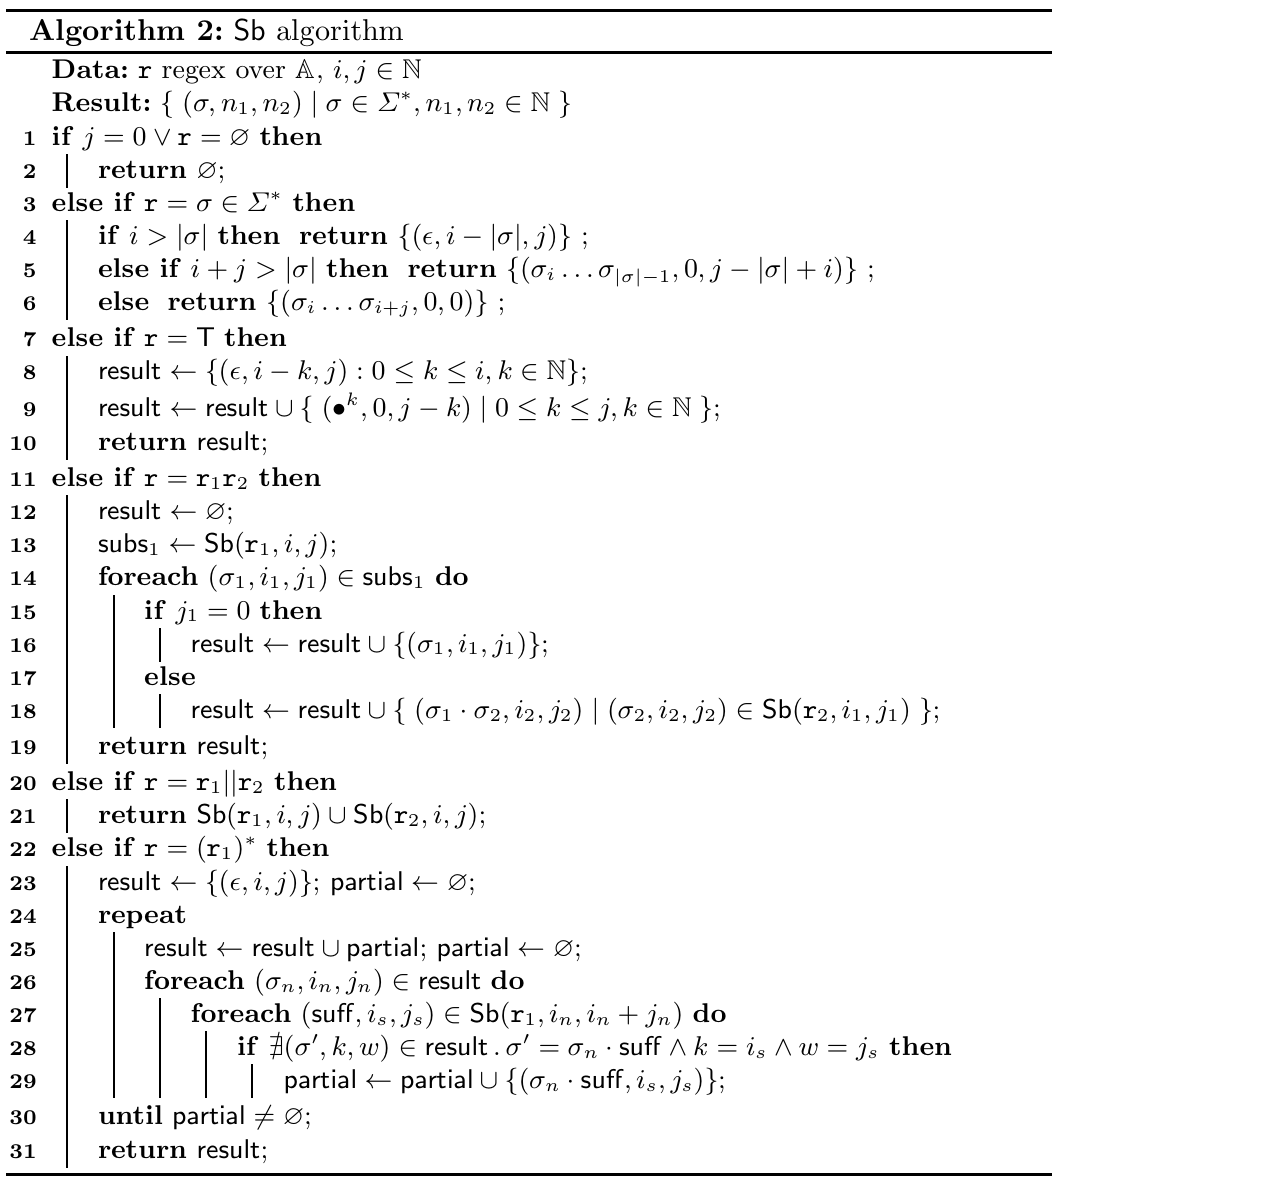
\includegraphics[width=\textwidth]{images/tarsis-SB-algo.png}\hfill
\end{figure}


\newpage
\subsubsection*{Replace}
\begin{figure}[H]
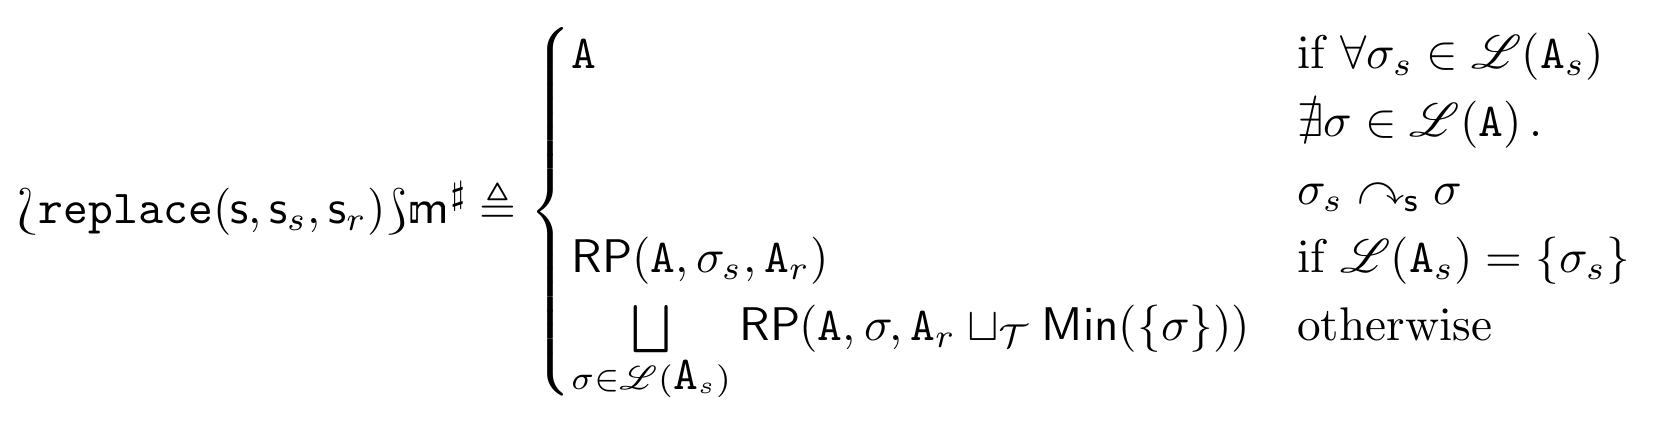
\includegraphics[width=\textwidth]{images/tarsis-replace.png}\hfill
\end{figure}

\begin{figure}[H]
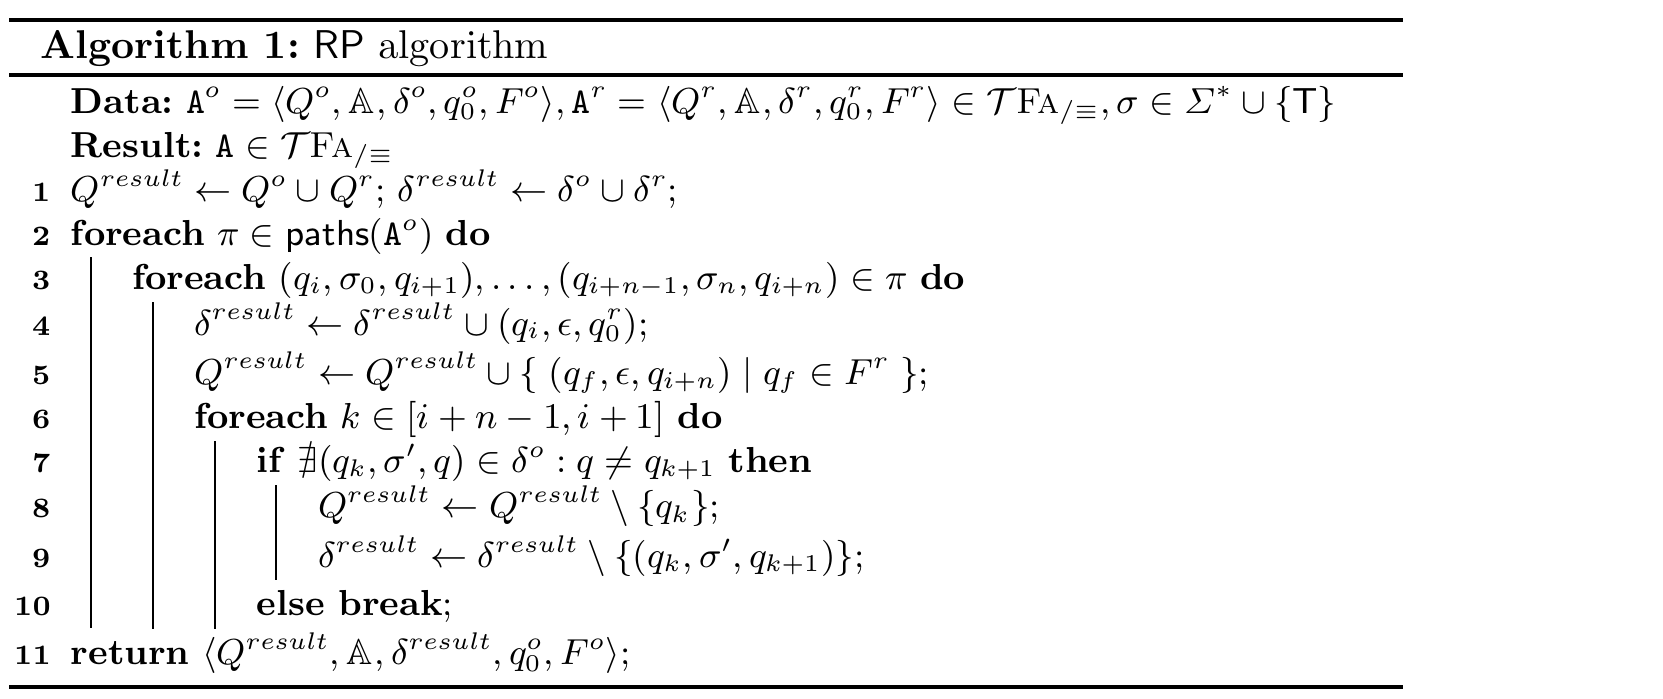
\includegraphics[width=\textwidth]{images/tarsis-RP-algo.png}\hfill
\end{figure}




\newpage
\subsection{Оператор расширения}
Важным методом является оператор расширения (widening). Именно благодаря ему удается завершать циклы за конечное время, создавая аппроксимацию. Рассмотрим пример того, как это реализованно

\begin{lstlisting}[caption={Пример применения widening}]
function f(v) {
    res = "";
    while(?) res = res + "id = " + v;
    return res;
}
\end{lstlisting}

Автомат, задающий значения res в начале второй итерации цикла while, выглядит так:
\begin{figure}[h]
    \centering
    \begin{tikzpicture}[->, >=stealth', shorten >=1pt, auto, node distance=3cm, semithick]
        \node[state, initial, accepting] (q0) {$q_0$};
        \node[state, right of=q0] (q1) {$q_1$};
        \node[state, right of=q1, accepting] (q2) {$q_2$};
        
        \path (q0) edge node[above] {id = } (q1)
                (q1) edge node[above] {$\top$} (q2);
    \end{tikzpicture}
\end{figure}

В конце второй итерации вот так:
\begin{figure}[h]
    \centering
    \begin{tikzpicture}[->, >=stealth', shorten >=1pt, auto, node distance=3cm, semithick]
        \node[state, initial] (q0) {$q_0$};
        \node[state, right of=q0] (q1) {$q_1$};
        \node[state, right of=q1, accepting] (q2) {$q_2$};
        \node[state, right of=q2] (q3) {$q_3$};
        \node[state, right of=q3, accepting] (q4) {$q_4$};
        
        \path (q0) edge node[above] {id = } (q1)
                (q1) edge node[above] {$\top$} (q2)
                (q2) edge node[above] {id = } (q3)
                (q3) edge node[above] {$\top$} (q4);
    \end{tikzpicture}
\end{figure}

Далее, для этих двух автоматов приминяем саму операцию расширения. Алгоритм такой:
\begin{itemize}
    \item Делаем union для этих автоматов:
    \begin{figure}[h]
        \centering
        \begin{tikzpicture}[->, >=stealth', shorten >=1pt, auto, node distance=3cm, semithick]
            \node[state, initial, accepting] (q0) {$q_0$};
            \node[state, right of=q0] (q1) {$q_1$};
            \node[state, right of=q1, accepting] (q2) {$q_2$};
            \node[state, right of=q2] (q3) {$q_3$};
            \node[state, right of=q3, accepting] (q4) {$q_4$};
            
            \path (q0) edge node[above] {id = } (q1)
                    (q1) edge node[above] {$\top$} (q2)
                    (q2) edge node[above] {id = } (q3)
                    (q3) edge node[above] {$\top$} (q4);
        \end{tikzpicture}
    \end{figure}

    \newpage
    \item Стейты, у которых исходящие пути длины 2 совпадают, объединяем. В данном случае $q_0$ и $q_2$ оба принимают $id = \top$, и потому склеиваются в одну вершину:
    \begin{figure}[h]
        \centering
        \begin{tikzpicture}[->, >=stealth', shorten >=1pt, auto, node distance=3cm, semithick]
            \node[state, initial, accepting] (q0) {$q_0, q_2$};
            \node[state, right of=q0] (q1) {$q_1$};
            \node[state, below of=q1] (q3) {$q_3$};
            \node[state, right of=q3, accepting] (q4) {$q_4$};
            
            \path (q0) edge node[above] {id = } (q1)
                    (q0) edge node[right] {id = } (q3)
                    (q1) edge[bend left] node[above] {$\top$} (q0)
                    (q3) edge node[above] {$\top$} (q4);
        \end{tikzpicture}
    \end{figure}

    В общем случае длину пути для склейки вершин можно регулировать, чем она больше, тем точнее результат, однако и размер автомата больше
    \item Минимизируем полученный автомат:
    \begin{figure}[h]
        \centering
        \begin{tikzpicture}[->, >=stealth', shorten >=1pt, auto, node distance=3cm, semithick]
            \node[state, initial, accepting] (q0) {$q_0$};
            \node[state, right of=q0] (q1) {$q_1$};
            
            \path (q0) edge node[above] {id = } (q1)
                    (q1) edge[bend left] node[above] {$\top$} (q0);
        \end{tikzpicture}
    \end{figure}
\end{itemize}

Теперь заметим, что полученный автомат является неподвижной точкой. Для этого попробуем проделать ещё одну итерацию цикла. После объединения автоматов в начале и конце цикла получаем такой:

\begin{figure}[h]
    \centering
    \begin{tikzpicture}[->, >=stealth', shorten >=1pt, auto, node distance=3cm, semithick]
        \node[state, initial, accepting] (q0) {$q_0$};
        \node[state, right of=q0] (q1) {$q_1$};
        \node[state, right of=q1, accepting] (q2) {$q_2$};
        
        \path (q0) edge node[above] {id = } (q1)
                (q1) edge[bend left] node[above] {$\top$} (q0)
                (q1) edge node[above] {$\top$} (q2);
    \end{tikzpicture}
\end{figure}

Склеивать вершины не придется, однако при минимизации $q_0$ и $q_2$ станут одной, то есть получим начальный автомат, что означает отсутствие изменений и значит можно остановиться 

Доказано~\cite{widening}, что такой алгоритм расширения соответствует условиям овер-аппроксимации